\documentclass[paper=a4, fontsize=11pt]{scrartcl}

\usepackage[T1]{fontenc}
\usepackage{fourier}
\usepackage[utf8]{inputenc}

\usepackage[english]{babel}															% English language/hyphenation
\usepackage[protrusion=true,expansion=true]{microtype}	
\usepackage{amsmath,amsfonts,amsthm} % Math packages
\usepackage[pdftex]{graphicx}	
\usepackage{url}
\usepackage{abstract}
\usepackage{tabularx}
\usepackage{float}

%%% Custom sectioning
\usepackage{sectsty}
\allsectionsfont{\centering \normalfont\scshape}

%%% Custom headers/footers (fancyhdr package)
\usepackage{fancyhdr}
\pagestyle{fancyplain}
\fancyhead{}											% No page header
\fancyfoot[L]{}											% Empty 
\fancyfoot[C]{}											% Empty
\fancyfoot[R]{\thepage}									% Pagenumbering
\renewcommand{\headrulewidth}{0pt}			% Remove header underlines
\setlength{\headheight}{13.6pt}

%%% Equation and float numbering
\numberwithin{equation}{section}		% Equationnumbering: section.eq#
\numberwithin{figure}{section}			% Figurenumbering: section.fig#
\numberwithin{table}{section}				% Tablenumbering: section.tab#

%%% Maketitle metadata
\newcommand{\horrule}[1]{\rule{\linewidth}{#1}} 	% Horizontal rule

\title{
		%\vspace{-1in} 	
		\usefont{OT1}{bch}{b}{n}
		\normalfont \normalsize \textsc{Luleå University of Technology} \\ [25pt]
		\horrule{0.5pt} \\[0.4cm]
		\huge Algorithms and Data Structures - Lab 3 \\
		\horrule{2pt} \\[0.5cm]
}
\author{Course: D0012E \\ \\ 
		\normalfont 								\normalsize
        Marcus Lund (amuulo-4) \\\normalfont\normalsize Edvin Åkerfeldt (edvker-4)\\\normalfont\normalsize Samuel Karlsson (samkar-4)\\[-3pt]		\normalsize
        \today
}
\date{}

%%% Begin document


\begin{document}
\maketitle
\centerline{Second submission.}
\begin{figure}[h!]
  \centering
    
\includegraphics[width=1\textwidth]{algorithm}
\end{figure}
\newpage

\begin{abstract}
In this report the runtime of Dijkstra’s algorithm is analysed with different number of connections on on each node and different "D" sizes ("D" is the D in D-arr heap). The trend shows that a bigger graph results in a longer runtime. The best runtime were when "D" was about 13 thousand.
\\

Generally the tests we ran were very case sensitive. The runtime differs a lot between worst and best case. The time we used was an average of multiple testes to minimize the effect from best and worst case tests.  
\end{abstract}

\tableofcontents
\newpage

\section{Introduction}
In this report a lab on Dijkstra’s algorithm is presented. The lab was done in the course "algorithms and computer structure". The goal for the lab was to see how the runtime is effected on different sizes of "D" and different number of connections to each node.

\subsection{Language}
We chose to use Java as our programming language of choice over other languages, because it is a language the we are comfortable to work with. Java is also one of the better optimized languages.

\subsection{Implementation}
Implementing Dijkstra’s algorithm is a challenge because the graphs representation have a huge influence on Dijkstra’s algorithms runtime.

 We chose to use a class representation of the graph. The class implementaion is in some regard straight forward and logical but has a clear disadvantages when it comes to memory consumption. When the graph grows its memory usage grows very fast.
\\

The hardest part of implementating the Dijkstra’s algorithm is to find a way to add the new nods to the added ones without adding the same node twice. To solved that problem we used an array where we stored the added nodes, distance to node and the preceding node.


\section{Test procedure}
The tests were ran several times with different sizes "D" and edges. We ran the testes multiple times and tock the averages time.
\\

We ran tow tests, one were the "D" value differ from $1 000-20 000$ and $10 000$ nodes and $40 000$ edges. In the outer test we weried the edge numbers $10 000-40 000$ and $10 000$ and  "D" at $1000$. 
\\

The tests that were run are listed in \ref{Testing sets}.
\section{Result}
\begin{table}[]
\centering
\caption{Testing sets}
\label{Testing sets}
\begin{tabular}{lllll}
Nodes & Edges & D \\
40000 & 40000 & 2-2000 \\
40000 & 80000 & 2-2000 \\
80000 & 80000 & 2-2000 \\
80000 & 160000 & 2-2000 \\
40000 & 40000 & 1000 \\
40000 & 60000 & 1000 \\
40000 & 80000 & 1000 \\
40000 & 100000 & 1000 \\
\end{tabular}
\end{table}

\begin{figure}
  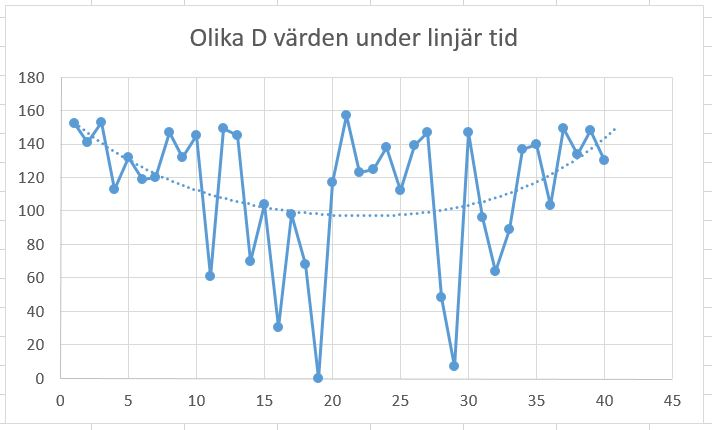
\includegraphics[width=\linewidth]{Average_of_diffrent_d_values.jpg}
  \caption{Different sizes of $d$. Time is on the y-axes and the value of $d$ on the x-axes.}
  \label{fig:result}
\end{figure}

\begin{figure}
  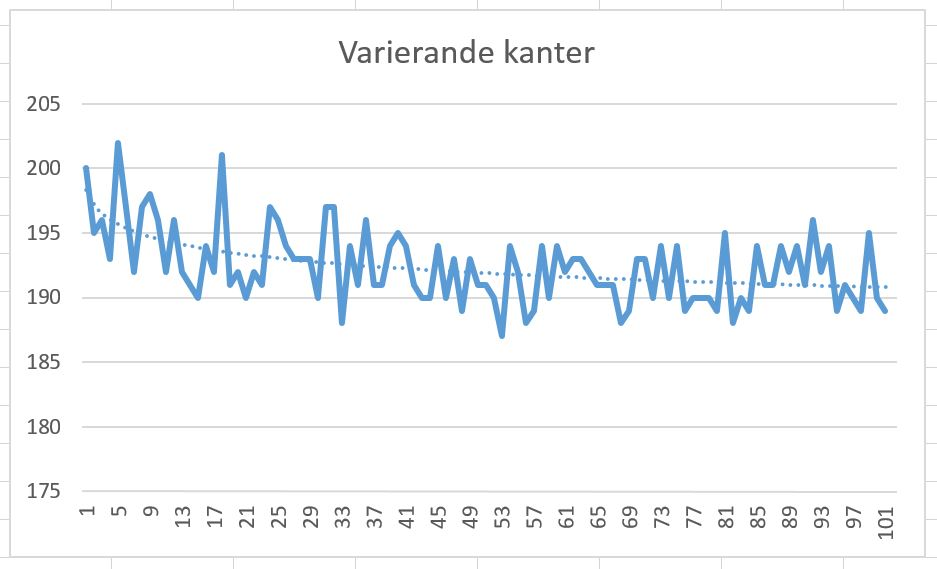
\includegraphics[width=\linewidth]{varierande_kanter.jpg}
  \caption{Different amount of edges. Runtime on the y-axes and size of edges on the x-axes.}
  \label{fig:result2}
\end{figure}

When increasing the value $d$ we see an increment in time.
Also with more edges and more nodes we get a bigger graph and thus it takes a longer time to calculate.

In graph \ref{fig:result} there is 4 different coloured bars where blue is $d=4$, orange $d=8$, grey $d=16$ and yellow is $d=31$. The bottom axis describes '$nodes$ \& $edges$' and the vertical axis describes the average time. We can see from the graph that $d$ has an impact of the average time when it is increased. But the number of edges has an even greater impact.

\section{Discussion}
Our theoretical assumption is that $d$ does affect the runtime depending on the relation between the number of nodes and the number of children of each node. According to the graph \ref{fig:result}, we see the behaviour of a smaller value of $d$ results in a large runtime. While $d$ increases the runtime gets smaller before reaching a point where the time does increase. This indicates that there is an optimum value of $d$ to achieve the fastest runtime.\\

Our thought is that when we reach the point after the $d$ sweet-spot, we have a lot more paths to loop through to find $b$, which may increase the total runtime. We think this is the answer to why the time increases.\\

As we look on the graph \ref{fig:result2}, we see some behaviour that decreases while the amount of edges gets lager. Although the behaviour is only in the beginning of out graph, we do not think this has any larger impact than $d$. 
Increasing the vertices has a smaller effect than the change while using different of $d$. \\
\\~\\
We see that if we use different $d$ values, we will find a sweet spot in order to achieve the fastest runtime. If we vary the vertices, we don't see as big of an impact on the runtime.
\\
PSEUDO of BIG O:\\
$
Worst case = vertices.length $*$ (adjesont.size $*$ log_d(vertices.length) + log_d(vertices.length))
$\\~\\
We would also like to pint out that we are no masters of programming. We might have some minor bugs in out program that caused the different values in out graphs. Our results gives us an assumption to consider, and the result might might differ from out implementation to others. When running these test, we used a Windows computer doing other stuff as well as running our tests. This is a highly cause of why our graphs look like they do.
%%% End document
\end{document}
